\chapter{Einleitung}
	\label{Kap1}
Die Einleitung gibt Lesenden eine Übersicht über den Inhalt, anfangend mit einer Beschreibung des technischen Problemfelds und dessen Einordnung im globalen Kontext, über die Feststellung der Ausgangssituation, hin zur Ausformulierung der Aufgaben und Zielen und endend mit der Erklärung des Aufbaus der Arbeit.

\section{Problemumfeld}		% (Einführung in den übergeordneten Themenbereich, damit z.B. Studierende verstehen, 	worum es geht. Was ist das Problem, das Sie lösen sollen? Was ist daran neu?)
	Anthropogene Treibhausgasemissionen (\ac{GHE}) weltweit führen laut Expertise der Mehrheit aller Klimaforscher*innen zu einem globalen Klimawandel mit Konsequenzen für alle. \cite{IPCC_Climate_Change_2007} Die verheerendsten Folgen treffen jedoch überwiegend Länder, die den Klimawandel am wenigsten verursachen. Eine Lösung mit holistischem Ansatz ist eine radikale Energiewende, mit dem Ziel den gesamten Energiesektor möglichst bedarfsorientiert, emissionsfrei und nachhaltig erneuerbar zu gestalten. Die Energiewende vollzieht sich in einem gesellschaftlichen Wandel und einem grundlegenden Strukturwandel des Energiesektors in den Teilsektoren Mobilität, Strom und Wärme. \\

	Als Teil der Energiewende wachsen die technischen Anforderungen an das elektrische Netz, um die Versorgungssicherheit und Spannungsqualität zu gewährleisten, wie zum Beispiel die Menge bereitstellbarer Regelleistung, Energiespeicherkapazitäten, Übertragungskapazitäten und Kommunikationsmöglichkeiten von Erzeugungs- und Verbrauchseinheiten für intelligente Energiemanagementsysteme. \\
    
    Die genannten Anforderungen wachsen zum Einen durch den sukzessiven Ausbau  fluktuierender, dezentraler Erzeugungsanlagen elektrischer Energie wie Windräder und Photovoltaikanlagen, welche konventionelle, thermische Großkraftwerke ersetzen. Zum Anderen begründen sie sich im zu erwartenden Wachstum des Stromsektors durch den stattfindenden Wandel hin zur Elektrifizierung des Mobilitätssektors, was neben dem Ausbau des öffentlichen Personen-(Nah-)Verkehrs und weniger, besser ausgelasteter Automobilnutzung wegweisend für eine sozialere, nachhaltigere Wirtschaftsweise ist. \cite{FraunhoferISI_Emobility_2011} Im Mobilitätssektor wurden 2015 durch mehrheitlichen Einsatz von Verbrennungsmotoren ca. 14 \% der \ac{GHE} und die Hälfte der gesundheitsschädlichen Stickstoffoxid-Emissionen in Deutschland emittiert. \cite{UBA_GHE} \cite{UBA_NOx} \cite{FraunhoferISI_Emobility_2011}\\ 






%  Der Stromsektor wird derzeit zu etwa 2/3 von konventionellen, thermischen Großkraftwerken versorgt, welche durch den Ausbau vieler, kleinerer, dezentraler Erzeugungsanlagen wie Windräder und Solaranlagen ersetzt werden können. Diese sind nachhaltig ressourcenschonender, fluktuieren allerdings in der Erzeugung, womit die Anforderungen für bereitstellbare Regelleistung, Energiespeicher, Übertragungskapazitäten und Kommunikationsmöglichkeiten von Erzeugungs- und Verbrauchseinheiten für intelligente Energiemanagementsysteme wachsen

  

% Klimawandel und Energiewende
%	Um die verheerendsten Folgen des anthropogenen Klimawandels zu verhindern, ist die Reduktion von Treibhausgasemissionen (\ac{GHE}) notwendig. Dies kann durch geringere Verbräuche, nachhaltigere Technologien, wie beim Umstieg auf erneuerbare Energien, und gesteigerte Effizienz erreicht werden, wobei letzteres einen Rebound-Effekt erzeugt. Klimaforscher*innen und -schützer*innen raten zu einer radikalen Energiewende, um den gesamten Energiesektor emissionsfrei(er) zu gestalten.\\
	
% Mobilitätssektor
%	Der Mobilitätssektor verursachte überwiegend durch Verbrennungsmotoren 2015 ca. 14 \% der \ac{GHE} und die Hälfte der gesundheitsschädlichen Stickstoffoxid-Emissionen in Deutschland. Diese können durch den Ausbau des öffentlichen Personen-(Nah-)Verkehrs, weniger und besser ausgelastete Automobilnutzung und den Umstieg auf Elektro-Motoren reduziert werden, was einen erhöhten Strombedarf mit sich bringt.\cite{UBA_GHE} \cite{UBA_NOx} \cite{FraunhoferISI_Emobility_2011}\\ 

% Stromsektor
%	Der Stromsektor wird noch von konventionellen, thermischen Großkraftwerken dominiert, welche durch den Ausbau vieler, kleinerer, dezentraler Erzeugungsanlagen wie Windräder und Solaranlagen ersetzt werden können. Diese sind nachhaltig ressourcenschonender, fluktuieren allerdings in der Erzeugung und sind somit nicht regelbar.\\
   %Momo: nicht regelbar ist doch bullshit - die Erzeugung selbst kann (meistens) nicht gescheit geregelt werden

% Netzanforderungen
%	Mit diesem grundlegenden Strukturwandel wachsen die Anforderungen an Energiespeicher, Transportkapazitäten des elektrischen Netzes und Kommunikationsmöglichkeiten von Erzeugungs- und Verbrauchseinheiten. Ein überregionales Energiemanagement durch Laststeuerung in einem intelligenten Stromnetz wird somit zunehmend wichtiger. \\
%Momo: dem grundlegend notwendigen Strukturwandel (also der passiert zwar grade aber ich finde den Satz zu schwammig)



%	Die Nutzung von Verbrennungsmotoren hat die folgenden Auswirkungen auf Mensch und Umwelt:
%	\begin{itemize}
%		\item Mehr Arbeit(splätze) aufgrund der höheren Kompexizität eines V-Motors gegenüber eines E-Motors
%		\item Resourcenabhängigkeit von fossilem, endlichem Brennstoff Erdöl oder genug verfügbarer fruchtbar Ackerfläche für Bio-Treibstoff
%		\item Resourcenkonflikte in einer konkurrenzbasierten Marktwirtschaft wie Landgrabbing und Kriege
%		\item Gesundheitliche Folgeschäden, unter anderem durch Feinstaub und Stickoxyde [Quelle XYZ]
%		\item Kurzfristig weniger Ausbau des elektrischen Netzes und der Ladeinfrastruktur für E-Autos nötig
%		\item Aktuell gute Tankstelleninfrastruktur verfügbar ohne Berücksichtigung der Produktionsbedingungen
%		\item Langfristig eventuell mehr Aufwand für Erhaltung der Netzstabilität mangels Regelleistung aus leistungsstarken, intelligent vernetzten Fahrzeugbatterien
%	\end{itemize}
%
%	Für eine sozialere und nachhaltigere Wirtschaftsweise ist zum einen die Umstellung von Fahrzeugen hin zu elektrischen Antrieben wegweisend, da sie kurz- bis mittelfristig die Technologie mit dem größten Umsetzungspotential im Mobilitätssektor ist, zum anderen ein zunehmend wachsender Anteil erneuerbarer Energien im gesamten Energiesektor.\cite{FraunhoferISI_Emobility_2011} \\



\section{Ausgangssituation}
	%Stand der Technik (Überblick über aktuelle Literatur zu Ihrem Thema, d.h. Bücher, Fachartikel in Zeitschriften wie "atp", "at" o.a. Dabei sollen Ideen, Konzepte, Algorithmen o.ä. aus anderen wissenschaftlichen Arbeiten zusammengefasst werden, die für Ihre Arbeit interessant sein sind oder von denen sich Ihre Arbeit abgrenzt, keine pure Marktübersicht)

% Nationale Enwicklungsplan E-Mobilität\\	
	Der Nationale Entwicklungsplan (NEP) der Bundesregierung sieht vor, 1 Mio. E-Autos bis 2020 und 6 Mio. E-Autos bis 2030 auf deutsche Straßen zu bringen. Anhand der vom \ac{KBA} veröffentlichen Zahlen über zugelassene Elektrofahrzeuge in Deutschland, dargestellt in Abb. \ref{Abb:Efahrzeuge_Deutschland_2004_2017}, ist absehbar, dass das Ziel des NEP bis 2020 wahrscheinlich verfehlt wird. Unter Annahme eines näherungsweise konstanten Zuwaches bis 2020 wie im Zeitraum seit 2013 bis 2017, wären 2020 ca. 55.000 bis 60.000 E-Fahrzeuge statt der nach NEP vorgesehenen 1.000.000 Elektrofahrzeuge zugelassen. \cite{NEP_2009}\\
	
	\begin{figure}[h]
		\centering
		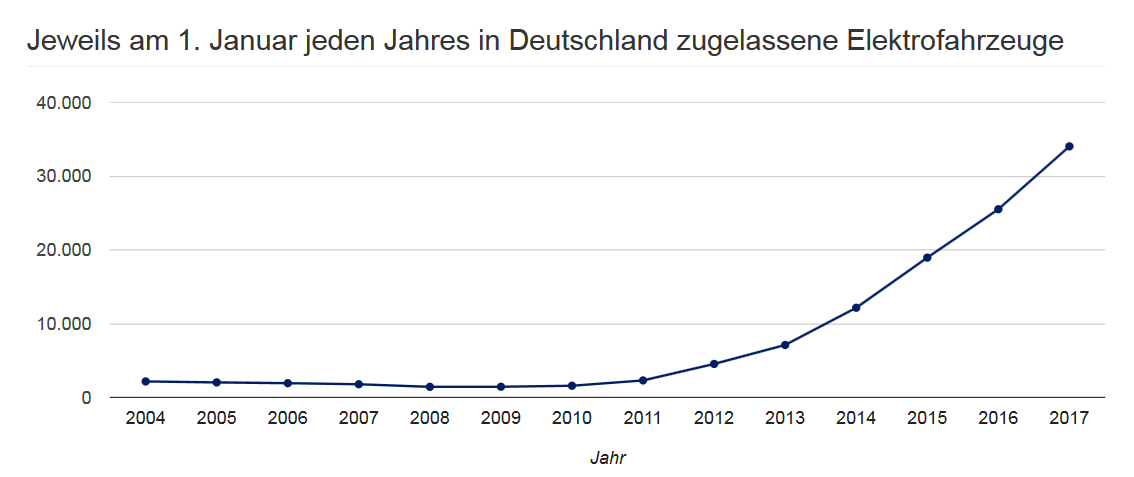
\includegraphics[width=14cm]{Efahrzeuge_Deutschland_2004_2017}
		\caption{Zugelassene E-Fahrzeuge in Deutschland von 2004 bis 2017 \cite{KBA_EAutos_Zulassungen} }
		\label{Abb:Efahrzeuge_Deutschland_2004_2017}
	\end{figure}
	
% Fördermittel
	Ein Flaschenhals bei der Elektrifizierung des automobilen Individualverkehrs ist die geringe Verfügbarkeit von Ladepunkten, weshalb der Ausbau der Ladeinfrastruktur durch Fördermittel des Bundesministeriums für Umwelt, Naturschutz, Bau und Reaktorsicherheit (BMUB) und des Bundesministeriums für Verkehr und digitale Infrastruktur (BMVI) begünstigt wird.\cite{BMVI_Frderrichtlinie_Ladeinfra}\\
% Momo: man braucht Ladepunkte um die Versorgung für die Autos zu gewährleisten - da könnts hacken bei laien

	\subsection{Projekt Energieverbundinsel}
		Auf Gebäude C der Hochschule Mannheim ist eine PV-Anlage mit einer Peakleistung von 20,145 kWp installiert mit einem durschnittlichen Jahresertrag von ca. 20.000 kWh. \\  %NOTE REF CITE XYZ
        % Der elektrische Verbrauch der gesamten Hochschule liegt bei ca. XYZ kWh pro Jahr.\\
		
		Im Sommersemester 2015 wurde im Rahmen einer Studienarbeit an der Hochschule Mannheim erstmalig ein Konzept für das Projekt Energieverbundsystem \glqq Energieinsel Mannheim\grqq \space erstellt. Mit beispielhaften Erzeuger- und Verbrauchersystemkomponenten wird eine Energieflussberechnung durchgeführt. Die betrachteten Systemkomponenten sind ein PV-System mit 25 kW Peakleistung, eine Lithium-Batterie mit ca. 27,5 kWh Speicherkapazität und 80\% \ac{DOD} mit zwei parallelen bidirektionalen Wechselrichtern mit einer Gesamtleistung von ca. 10 kW, Ladeinfrastruktur für Elektrofahrzeuge mit ca. 10,3 kW maximaler Ladeleistung, ein Elektrolyseur zur Wasserstoffgewinnung und eine Brennstoffzelle.\cite{STA_Oliver_Kersten_2015}\\
%Momo: -STC ne erklärung oder ne cite zu welche conditionas das sind

		Im Wintersemester 2017/18 wurde im Rahmen einer Bachelorthesis angelehnt an die \ac{HOAI}, eine Grundlagenermittlung, Vorplanung und Entwurfsplanung für die \glqq Errichtung einer Energieverbundinsel mit teilautarker Ladeinfrastruktur für Elektrofahrzeuge\grqq \space  erstellt. Die maximal angenommene Ladeleistung für E-Fahrzeuge beträgt 50 kW. Das angesetzte Budget von 50.000 EUR wurde leicht überschritten.\cite{BA_Chris_Ong_2017}\\
		
		Die geplante Energieverbundinsel mit PV-Speicher und Pufferbatterie besitzt die Grundvoraussetzungen für eine smarte teilautarke Betriebsweise mit implementiertem \ac{EMS} für experimentelle Tests in der Praxis.
% Momo: Normalmensch könnte bei den Worten smart und micogrid hängen


\section{Aufgaben und Ziele}
	% (Was ist das Ziel Ihrer Arbeit? Welche Aufgaben sind im Einzelnen zum Erreichen dieses Ziels zu bearbeiten?)
	%Zum Besseren Verständnis sollte bereits hier eine grafische Darstellung des zu automatisierenden Systems bereitgestellt werden. 
	Mit dieser Thesis wird das Ziel verfolgt die Planung der Errichtung einer Energieverbundinsel mit teilautarker Ladeinfrastrukur weiter zu entwickeln. Dafür wird ein Konzept für ein Energiemanagementsystem erstellt mit einer Übersicht der notwendigen Systemanforderungen zur intelligenten Steuerung und Überwachung der Ladetechnik für E-Fahrzeuge und Pufferbatterien.\\
	
	Mithilfe simulierter Energieflussberechnungen für verschiedene Szenarien sollen Handlungsempfehlungen für die Dimensionierung und Betriebsweise der Energieverbundinsel gegeben werden. Hierzu werden theoretisch erreichbare Autarkiegrade für die Ladeinfrastruktur in Abhängigkeit von Ladeleistung, PV-Leistung und Kapazität der Pufferbatterie ermittelt. Für die Simulationen wird eine Testumgebung in Matlab-Code geschrieben, um die Untersuchung weiterer Szenarien zu erleichtern. \\
	
%	Für eine Optimierung von Kosten, Aufwand und/oder Umweltschäden werden verschiedene Alternativoptionen zu der in \cite{BA_Chris_Ong_2017} aufgestellten Entwurfsplanung vorgestellt. Hierfür werden u.A. verschiedene verfügbare Batterietechnologien für den Einsatz als stationäre Pufferbatterien verglichen. \\
	
%	Pflichtenheft:
%	\begin{itemize}
%		\item Vorgaben: Ladeleistung * 120 \% Reserve < 50 kW 
%		\item Vorgaben: 3 Autos, 2 Roller/Motorräder, 5 Bikes
%		\item Konzept Energiemanagement
%		\item Zentrale Monitoring- und Steuerungseinheit entwerfen (Welche Daten werden geloggt, wie aufbereitet, wie angezeigt, was kann gesteuert werden, welche Kommunikationstechnik wird verwendet)
%		\item Überblick Systemkomponenten
%		\item Energieflussberechnung, Prognose
%		\item Mögliche Abrechnungssysteme bewerten ???
%		\item Kostenreduktion, Alternativoptionen ???
%	\end{itemize}

% Weitere Möglichkeiten:
%		Teststation für Energie-/Lastenmanagement und Kommunikation im IoT mit Option zur Fahrbatterieentladung
%		Ladeanschlusstechnik in open source (Anwendung des XYZ Protokolls, s. Signalisierung Typ 2 bzw. „Configuration FF“ - PLC-basiertes Layer-1-Kommunikationsprotokoll über Combo Typ-2-Stecker )
%		ev. selbstgebautes Batterypack https://batterybro.com/pages/18650-battery-pack

	

%	Energieverbundinsel
%		Energieflüsse\\
%			- Bilanzierung, geschätzte/r Erzeugung/Verbrauch
%			- Monitoring (Momentanwerte, Tagesverläufe, Wochen-/Monats-/Jahreswerte)\\
%				- - PV-Anlage\\
%				- - Akkus\\
%				- - Temperatur \\
%				- - Ladeverbrauch\\
%				- - Restliche Hochschule\\
%			- Controlling\\
%				- - Akkus\\
%				- - Heizsystem für Akkus- und Ladegeräte\\		


%		Kostensenkung\\
%			Holz-/Metallcontainer\\
%			PV-Anlage statt hoher Stromrechnung\\
%			Größer angelegte Batterie\\
%			Heizsystem für Batterie \\
%			Abrechnungssystem basierend auf OCPP\\


			

\section{Aufbau der Arbeit}
%	Orientierung an HOAI Leistungsphasen(LP) 1 bis 3.
%	
%	LP1: \\
%		- Technische Grundlagen zu bestehenden Ladesystemen verschiedener Fahrzeugtypen, Batterietypen, PV-Anlagen.\\
%		- Bestandsaufnahme Fahrzeuge, Standortanalyse, Zielvorgaben, Definition Workflow\\
%	LP2:\\
%		- Auslegung der Anlage (Ladeleistung, Batteriekapazität/-leistung, etc.)\\
%	LP3:\\
%		- Entwurfsplanung, Modelle erstellen, mit Anbietern/Herstellern beraten, Kostenrechnung\\
	Der Arbeit vorangestellt sind ein Abstract, das Ziele und Ergebnisse der Arbeit zusammenfasst und ein Abkürzungsverzeichnis.\\
    
	Die eigentliche Thesis beginnt mit einer Einleitung in Kapitel \ref{Kap1}, in der das Problemumfeld, die Ausgangssituation, die Aufgaben und Ziele und der Aufbau der Arbeit beschrieben werden. In Kapitel \ref{Kap2} wird die Basis für den Hauptteil der Arbeit geschaffen. Neben den technischen Grundlagen und Rahmenbedingungen wird dort das methodische Vorgehen beschrieben.\\
	
	In der ersten Hälfte des Hauptteils, Kapitel \ref{Kap3}, wird das Konzept der Energieverbundinsel und ein zugehöriges Energymanagementsystem entworfen.	In der zweiten Hälfte des Hauptteils, Kapitel \ref{Kap4}, werden Randbedingungen für verschiedene Szenarien für Energieflussberechnungen der Energieverbundinsel festgelegt, die Funktionsweise eines programmierten Simulationstools vorgestellt und die Ergebnisse der simulierten Energieflüsse wiedergegeben.\\
	
    In Kapitel \ref{Kap5} werden die Simulationsergebnisse zusammengefasst, bewertet und Handlungsempfehlungen für die Dimensionierung und Betriebsweise daraus abgeleitet sowie ein Ausblick auf zukünftige Entwicklungen geschaffen. Die Ergebnisse der Arbeit und eine kritische Schlussbetrachtung werden in einem Fazit in Kapitel \ref{Kap6} zusammengefasst. \\
    
    Im Anschluss an die Kapitel finden sich Verzeichnisse für Literaturquellen, Tabellen, Abbildungen und Quellcodes. \\
	
    Im Anhang finden sich technische Spezifikationen wie z.B. Datenblätter, Rechenmethoden zur Ermittlung von PV-Ertragsleistungen anhand waagrecht auf den Grund treffender Globalstrahlungsdaten, eine Beschreibung des Smart Grid Architecture Model (SGAM) Frameworks und Codebeispiele der entwickelten Programme.
    
     % ... Mit Orientierumg am Smart Grid Architecture Model, welches in Anhang \ref{Kap:SGAM_aufbau} näher beschrieben wird
     %  ...wird eine Use Case Analysis für die Anwendung der Energieverbundinsel durchgeführt. Aufbauend auf der Usecase Analysis werden die für die Simulation notwendigen Funktionalitäten, Datenmodelle und Komponenten beschrieben. 
    
    